\documentclass[11pt]{article}
\usepackage[margin=0.7in]{geometry}
\usepackage{tikz,longtable,hyperref}
\setlength{\parindent}{0pt}\setlength{\parskip}{7pt}
\begin{document}
{\LARGE Pencil mathematical study: native preparation evidence}\\[5pt]
2026-10-29T22:47:16Z\\
Public synthetic known-answer mathematical research. Evidence observations only; no judgments, new cohort executions or qualification.

Zero executions refers to this named plan-only input, not historical experiments. Per-source software scopes are distinct and counts are never pooled.
\section*{Plan-only observations}
\begin{center}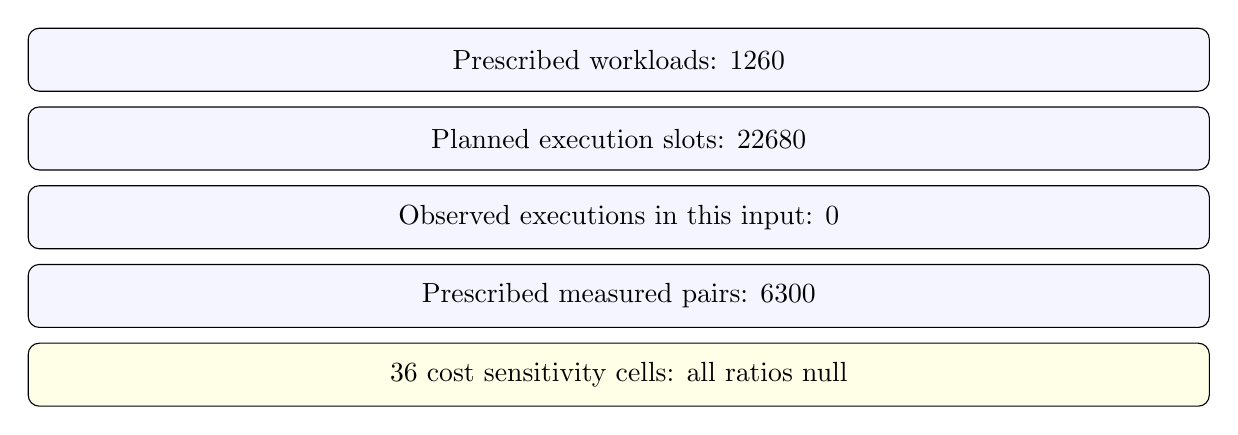
\begin{tikzpicture}
\node[draw,rounded corners,fill=blue!4,minimum width=15cm,minimum height=0.8cm] at (0,-0) {Prescribed workloads: 1260};
\node[draw,rounded corners,fill=blue!4,minimum width=15cm,minimum height=0.8cm] at (0,-1) {Planned execution slots: 22680};
\node[draw,rounded corners,fill=blue!4,minimum width=15cm,minimum height=0.8cm] at (0,-2) {Observed executions in this input: 0};
\node[draw,rounded corners,fill=blue!4,minimum width=15cm,minimum height=0.8cm] at (0,-3) {Prescribed measured pairs: 6300};
\node[draw,rounded corners,fill=yellow!10,minimum width=15cm,minimum height=0.8cm] at (0,-4) {36 cost sensitivity cells: all ratios null};
\end{tikzpicture}\end{center}
Diagram rather than a performance graph: this input contains no observed empirical ratios. Counts are read from source [plan]; no rates or uncertainty estimates are inferred.
Warmup execution slots prescribed: 3780. No empirical cost ratio is available in this snapshot. Software validation and prepared inputs do not constitute independent protocol, binary, resource or launch admission.
\section*{Scoped source observations}
\textbf{[first-gate]} Explicit user approval of larger FIRST gate only; cumulative budget, original deadline, IAM/controller, freeze and launch remain pending.\\
coefficient\_cap: 25000000\\
seconds\_per\_execution: 3600\\
targets: 60\\
\textbf{[native-preparation]} Current native preparation software and run-free parity only; actual frozen archive reextracted with current source543 instrument. Does not independently reproduce the instrument build.\\
archive\_reextracted: true\\
archive\_workloads: 1260\\
cohort\_slots: 22680\\
exact\_retained\_specs: true\\
software\_tests: 3\\
solver\_executions: 0\\
tests\_failed: 0\\
\textbf{[native-canonical]} Native canonical packaging/protocol software fixtures only; distinct from empirical targets and previous producer/analyzer suites.\\
clippy\_passed: true\\
empirical\_targets: 0\\
qualified\_cost\_ratio: null\\
tests\_failed: 0\\
tests\_passed: 28\\
\textbf{[native-report]} Native renderer software fixtures only; includes pdflatex PDF test and historical validation-scope preservation.\\
clippy\_exit\_code: 0\\
empirical\_targets: 0\\
tests\_failed: 0\\
tests\_passed: 8\\
\textbf{[instrument543]} Previously verified static ecbench build source543, separate from native tooling; plan-only checks and no solver execution.\\
archive\_targets: 1260\\
prepared\_plans: 9\\
solver\_executions: 0\\
source: "543a54b4b1c3be7052872af3ffe393a44c69a3c3"\\
\textbf{[root-full]} Source0cd test-only correction validation lane: full default-parallel release suite failed. Exact source-file hashes are retained in receipt; focused passes do not replace this result.\\
exit\_code: 101\\
failed: 2\\
ignored: 123\\
passed: 5275\\
\textbf{[root-focused]} Separate bounded serial reruns of the two failed tests from the exact same compiled binary; not a passing full-suite result.\\
allocator\_failed: 0\\
allocator\_passed: 1\\
exit\_code: 0\\
gpu\_failed: 0\\
gpu\_passed: 1\\
\section*{Evidence and limits}
No software test count is an empirical target count. Missing costs stay null. Resource authorization is limited to its explicit source scope; no budget, deadline, infrastructure approval or independent review is inferred. The prior 19:06 report and its Python generator remain historical artifacts; new reports use this native renderer.
\small
\textbf{[plan]} named plan-only input; not historical experiments\\
\texttt{/\allowbreak{}home/\allowbreak{}ec2-user/\allowbreak{}crypto-pencil-signed-graph-20261029/\allowbreak{}research/\allowbreak{}pencil\_large\_prime\_20261029/\allowbreak{}validation/\allowbreak{}accounting/\allowbreak{}aggregate/\allowbreak{}actual-plan-only-summary-final.json}\\
SHA256: \texttt{9c0d055e2af7f6f79ce201b9b0c2a22691da0af55e8f6f127acec7070bb7e665}\\
\textbf{[first-gate]} Explicit user approval of larger FIRST gate only; cumulative budget, original deadline, IAM/controller, freeze and launch remain pending.\\
\texttt{/\allowbreak{}home/\allowbreak{}ec2-user/\allowbreak{}crypto-pencil-signed-graph-20261029/\allowbreak{}research/\allowbreak{}pencil\_large\_prime\_20261029/\allowbreak{}protocol\_draft/\allowbreak{}accounting\_amendment\_20261029/\allowbreak{}first\_gate\_authorization.json}\\
SHA256: \texttt{e04f26d0cab6850f3c477e9521ea4359c46f64ec436ce899b3b4049867710600}\\
\textbf{[native-preparation]} Current native preparation software and run-free parity only; actual frozen archive reextracted with current source543 instrument. Does not independently reproduce the instrument build.\\
\texttt{/\allowbreak{}home/\allowbreak{}ec2-user/\allowbreak{}crypto-pencil-signed-graph-20261029/\allowbreak{}research/\allowbreak{}pencil\_large\_prime\_20261029/\allowbreak{}native\_preparation/\allowbreak{}validation/\allowbreak{}receipt.json}\\
SHA256: \texttt{46843c028008698dc4eaa47370191904cf274791402d8953e23868e725d62ea3}\\
\textbf{[native-canonical]} Native canonical packaging/protocol software fixtures only; distinct from empirical targets and previous producer/analyzer suites.\\
\texttt{/\allowbreak{}home/\allowbreak{}ec2-user/\allowbreak{}crypto-pencil-signed-graph-20261029/\allowbreak{}research/\allowbreak{}pencil\_large\_prime\_20261029/\allowbreak{}native\_canonical\_export/\allowbreak{}validation/\allowbreak{}receipt.json}\\
SHA256: \texttt{6695b0cd726256602178b45ae446992d5e15fcaa5de0b611c66f8ea6cb16f0c3}\\
\textbf{[native-report]} Native renderer software fixtures only; includes pdflatex PDF test and historical validation-scope preservation.\\
\texttt{/\allowbreak{}home/\allowbreak{}ec2-user/\allowbreak{}crypto-pencil-signed-graph-20261029/\allowbreak{}research/\allowbreak{}pencil\_large\_prime\_20261029/\allowbreak{}native\_review\_report/\allowbreak{}validation.json}\\
SHA256: \texttt{99dcf2a854b4bb7d3e02c010f4e19bee71f44f5d9036de5a9c1ee3b00f0ff034}\\
\textbf{[instrument543]} Previously verified static ecbench build source543, separate from native tooling; plan-only checks and no solver execution.\\
\texttt{/\allowbreak{}home/\allowbreak{}ec2-user/\allowbreak{}crypto-pencil-signed-graph-20261029/\allowbreak{}research/\allowbreak{}pencil\_large\_prime\_20261029/\allowbreak{}validation/\allowbreak{}instrument\_build\_40938439022/\allowbreak{}receipt.json}\\
SHA256: \texttt{59fd9e0e1f4573d9492bcca710b5351cd0175f788b197a7c82939e177ab1a1a1}\\
\textbf{[root-full]} Source0cd test-only correction validation lane: full default-parallel release suite failed. Exact source-file hashes are retained in receipt; focused passes do not replace this result.\\
\texttt{/\allowbreak{}home/\allowbreak{}ec2-user/\allowbreak{}crypto-pencil-signed-graph-20261029/\allowbreak{}research/\allowbreak{}pencil\_large\_prime\_20261029/\allowbreak{}validation/\allowbreak{}hash\_one\_ci\_20261029/\allowbreak{}correction.json}\\
SHA256: \texttt{2c83885fbefef25323bf968aefdb1ea96c1b67bdd4ed7dcae84cb7c5d68014fe}\\
\textbf{[root-focused]} Separate bounded serial reruns of the two failed tests from the exact same compiled binary; not a passing full-suite result.\\
\texttt{/\allowbreak{}home/\allowbreak{}ec2-user/\allowbreak{}crypto-pencil-signed-graph-20261029/\allowbreak{}research/\allowbreak{}pencil\_large\_prime\_20261029/\allowbreak{}validation/\allowbreak{}hash\_one\_ci\_20261029/\allowbreak{}correction.json}\\
SHA256: \texttt{2c83885fbefef25323bf968aefdb1ea96c1b67bdd4ed7dcae84cb7c5d68014fe}\\
\end{document}
